%%%%%%%%%%%%%%%%%%%%%%%%%%%%%%%%%%%%%%%%%%%%%%%%%%%%%%%%
% Este é um documento que servirá de modelo para
% os relatórios feitos na disciplina Circuitos Digitais
% 2016-2
%%%%%%%%%%%%%%%%%%%%%%%%%%%%%%%%%%%%%%%%%%%%%%%%%%%%%%%%%

\documentclass[12pt]{article}

\usepackage{sbc-template}
\usepackage[brazil,american]{babel}
\usepackage[utf8]{inputenc}

\usepackage{graphicx}
\usepackage{url}
\usepackage{float}
\usepackage{listings}
\usepackage{color}
\usepackage{todonotes}
\usepackage{algorithmic}
\usepackage{algorithm}
\usepackage{hyperref}
     
\sloppy


\title{Experimento 3\\ 
Circuitos Combinacionais: Mapa de Karnaugh}


\author{João Pedro Silva Sousa, 15/0038381\\
        André Carvalho Marques,  15/0005491
}


\address{Dep. Ciência da Computação -- Universidade de Brasília (UnB)\\
  CiC 116351 - Circuitos Digitais - Turma A
  \email{\{jpssousa97,marquandre228\}@gmail.com}
}

\begin{document} 
\maketitle

\selectlanguage{american}
 \begin{abstract}
   Presentation of Karnaugh map for simplification of Boolean logic functions up to 5 variables applied in combinational circuits (implementation of majority decision circuits, minority and equality verification).
 \end{abstract}
\selectlanguage{brazil}     
    
 \begin{resumo} 
  Apresentação do mapa de Karnaugh para simplicação de funções lógicas booleanas de até 5 variáveis aplicadas em circuitos combinacionais (implementação de circuitos de decisão de maioria, minoria e verificação de igualdade).
 \end{resumo}


\section{Introdução}
\label{sec:Introducao}

O mapa de Karnaugh (normalmente abreviado por mapa K, ou \textit{K map}, em inglês) é um método gráfico utilizado para converter uma tabela verdade de um circuito lógico ou simplificar uma equação lógica. Um mapa de Karnaugh pode ser utilizado em problemas que possuem um número qualquer de variáveis de entrada, porém normalmente problemas que envolvem uma quantidade maior que seis váriáveis não se mostram práticos para serem avaliados pelo mapa K.

Similar a uma tabela verdade, o mapa de Karnaugh fornece a mesma informação no que diz respeito às entradas e saídas de uma função lógica, porém o mapa K se mostra bem mais compacto, uma vez que cada linha de uma tabela verdade é representada por um quadrado em um mapa de Karnaugh.

Por mais complexa que seja uma função lógica booleana, ela pode ser escrita utilizando as operações básicas (conjunção, disjunção e negação). Uma função escrita por uma soma de produtos é dita na forma canônica disjuntiva (onde cada termo é chamado de produto padrão, produto canônico ou mintermo) e, analogamente, um produto de somas é dito na forma canônica conjuntiva (onde cada termo é chamado de soma padrão, soma canônica ou maxtermo).

\subsection{Objetivos}
\label{sec:Objetivos}

Apresentar o mapa de Karnaugh e sua utilidade para simplificação de funções booleanas de até cinco variáveis.

\subsection{Materiais} 
\label{sec:Materiais}
Neste experimento foram utilizados os seguintes materiais e equipamentos:
\begin{itemize}
    \item Painel Digital

    \item \textit{protoboard}
    
    \item Fios
    
    \item Portas Lógicas OR, AND e NAND
\end{itemize}

\section{Procedimentos experimentais}
\label{sec:Procedimentos}

Foi considerado um circuito de decisão de maioria com quatro entradas. A saída $X$ será 1 se, e somente se, a maioria das entradas for igual a 1. A função que representa o circuito descrito anteriormente é:

\begin{equation}
\label{eq:decisao_maioria}
    X = \bar{A}BCD + A\bar{B}CD + AB\bar{C}D + ABC\bar{D} + ABCD
\end{equation}

que pode ser simplificada para:

\begin{equation}
\label{eq:simp_decisao_maioria}
    X = AB(C + D) + CD(A + B)
\end{equation}

\subsection{Circuito de decisão de maioria}
\label{sec:CMaioria}

O circuito de decisão de maioria de quatro entradas foi implementado utilizando portas AND e OR, somente, como mostra a Figura~\ref{fig:circ_maioria}.

\begin{figure}[H]
    \centering
    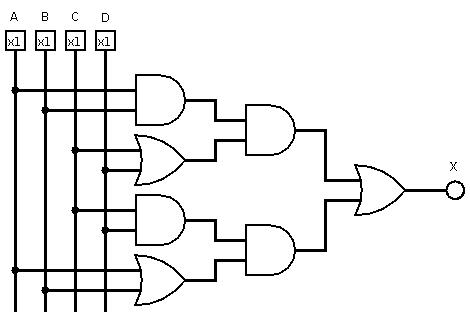
\includegraphics[width=.5\textwidth]{circuito_decisao_maioria.jpg}
    \caption{Circuito de decisão de maioria (4 entradas)}
    \label{fig:circ_maioria}
\end{figure}

A tabela verdade do circuito está representada abaixo, na Tabela~\ref{tab:circ_maioria}:

\begin{table}[H]
    \centering
    \caption{Tabela verdade - Circuito de decisão de maioria}

    \begin{tabular}{|c|c|c|c|c|}
    \hline
    \multicolumn{4}{c}{Entradas} & \multicolumn{1}{|c|}{Saída}\\
    \hline
    $A$ & $B$ & $C$ & $D$ & $X$\\
    \hline
    0 & 0 & 0 & 0 & 0\\
    \hline
    0 & 0 & 0 & 1 & 0\\
    \hline
    0 & 0 & 1 & 0 & 0\\
    \hline
    0 & 0 & 1 & 1 & 0\\
    \hline
    0 & 1 & 0 & 0 & 0\\
    \hline
    0 & 1 & 0 & 1 & 0\\
    \hline
    0 & 1 & 1 & 0 & 0\\
    \hline
    0 & 1 & 1 & 1 & 1\\
    \hline
    1 & 0 & 0 & 0 & 0\\
    \hline
    1 & 0 & 0 & 1 & 0\\
    \hline
    1 & 0 & 1 & 0 & 0\\
    \hline
    1 & 0 & 1 & 1 & 1\\
    \hline
    1 & 1 & 0 & 0 & 0\\
    \hline
    1 & 1 & 0 & 1 & 1\\
    \hline
    1 & 1 & 1 & 0 & 1\\
    \hline
    1 & 1 & 1 & 1 & 1\\
    \hline
    \end{tabular}
    \label{tab:circ_maioria}
\end{table}

O mapa de Karnaugh do circuito está mostrado na Tabela~\ref{tab:k_map_circ_maioria}

\begin{table}[H]
    \centering
    \caption{Mapa de Karnaugh - Circuito de decisão de maioria}

    \begin{tabular}{|c|c|c|c|c|}
    \hline
    $C$$D$ $A$$B$ & 00 & 01 & 11 & 10\\
    \hline
    00 & 0 & 0 & 0 & 0\\
    \hline
    01 & 0 & 0 & 1 & 0\\
    \hline
    11 & 0 & 1 & 1 & 1\\
    \hline
    10 & 0 & 0 & 1 & 0\\
    \hline
    \end{tabular}
    \label{tab:k_map_circ_maioria}
\end{table}


\subsection{Circuito de decisão de minoria}
\label{sec:CMinoria}

Foi implementado um circuito de decisão de minoria também de quatro entradas, utilizando apenas portas NAND. O circuito exibe a saída $Y$ igual a 1 se, e somente se, a minoria das entradas forem iguais a zero. A implementação do circuito na protoboard e utilizando o painel digital para aferir a saída segue o esquema representado na Figura~\ref{fig:circ_minoria}.

\begin{figure}[H]
    \centering
    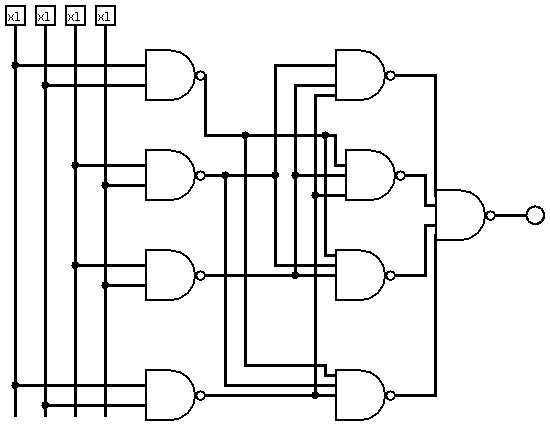
\includegraphics[width=.5\textwidth]{circuito_decisao_minoria.jpg}
    \caption{Circuito de decisão de minoria (4 entradas)}
    \label{fig:circ_minoria}
\end{figure}

A tabela verdade do circuito descrito acima está representada na Tabela~\ref{tab:circ_minoria}:

\begin{table}[H]
    \centering
    \caption{Tabela verdade - Circuito de decisão de maioria}

    \begin{tabular}{|c|c|c|c|c|}
    \hline
    \multicolumn{4}{c}{Entradas} & \multicolumn{1}{|c|}{Saída}\\
    \hline
    $A$ & $B$ & $C$ & $D$ & $Y$\\
    \hline
    0 & 0 & 0 & 0 & 1\\
    \hline
    0 & 0 & 0 & 1 & 1\\
    \hline
    0 & 0 & 1 & 0 & 1\\
    \hline
    0 & 0 & 1 & 1 & 0\\
    \hline
    0 & 1 & 0 & 0 & 1\\
    \hline
    0 & 1 & 0 & 1 & 0\\
    \hline
    0 & 1 & 1 & 0 & 0\\
    \hline
    0 & 1 & 1 & 1 & 0\\
    \hline
    1 & 0 & 0 & 0 & 1\\
    \hline
    1 & 0 & 0 & 1 & 0\\
    \hline
    1 & 0 & 1 & 0 & 0\\
    \hline
    1 & 0 & 1 & 1 & 0\\
    \hline
    1 & 1 & 0 & 0 & 0\\
    \hline
    1 & 1 & 0 & 1 & 0\\
    \hline
    1 & 1 & 1 & 0 & 0\\
    \hline
    1 & 1 & 1 & 1 & 0\\
    \hline
    \end{tabular}
    \label{tab:circ_minoria}
\end{table}

O mapa de Karnaugh do circuito está mostrado na Tabela~\ref{tab:k_map_circ_minoria}

\begin{table}[H]
    \centering
    \caption{Mapa de Karnaugh - Circuito de decisão de minoria}

    \begin{tabular}{|c|c|c|c|c|}
    \hline
    $C$$D$ $A$$B$ & 00 & 01 & 11 & 10\\
    \hline
    00 & 1 & 1 & 0 & 1\\
    \hline
    01 & 1 & 0 & 0 & 0\\
    \hline
    11 & 0 & 0 & 0 & 0\\
    \hline
    10 & 1 & 0 & 0 & 0\\
    \hline
    \end{tabular}
    \label{tab:k_map_circ_minoria}
\end{table}


\subsection{Circuito de verificação igualitária}
\label{CIgual}

Foi projetado um circuito de verificação igualitária que possui quatro entradas e exibe a saída $Z$ igual a 1 se, e somente se, a quantidade de 1's e 0's na entrada forem iguais, não importanto a ordem das entradas. O circuito foi implementado utilizando apenas portas NAND.

A tabela verdade do circuito descrito acima está representada na Tabela~\ref{tab:circ_igual}:

\begin{table}[H]
    \centering
    \caption{Tabela verdade - Circuito de decisão de maioria.}

    \begin{tabular}{|c|c|c|c|c|}
    \hline
    \multicolumn{4}{c}{Entradas} & \multicolumn{1}{|c|}{Saída}\\
    \hline
    $A$ & $B$ & $C$ & $D$ & $Z$\\
    \hline
    0 & 0 & 0 & 0 & 0\\
    \hline
    0 & 0 & 0 & 1 & 0\\
    \hline
    0 & 0 & 1 & 0 & 0\\
    \hline
    0 & 0 & 1 & 1 & 1\\
    \hline
    0 & 1 & 0 & 0 & 0\\
    \hline
    0 & 1 & 0 & 1 & 1\\
    \hline
    0 & 1 & 1 & 0 & 1\\
    \hline
    0 & 1 & 1 & 1 & 0\\
    \hline
    1 & 0 & 0 & 0 & 0\\
    \hline
    1 & 0 & 0 & 1 & 1\\
    \hline
    1 & 0 & 1 & 0 & 1\\
    \hline
    1 & 0 & 1 & 1 & 0\\
    \hline
    1 & 1 & 0 & 0 & 1\\
    \hline
    1 & 1 & 0 & 1 & 0\\
    \hline
    1 & 1 & 1 & 0 & 0\\
    \hline
    1 & 1 & 1 & 1 & 0\\
    \hline
    \end{tabular}
    \label{tab:circ_igual}
\end{table}

O mapa de Karnaugh do circuito está mostrado na Tabela~\ref{tab:k_map_circ_igual}

\begin{table}[H]
    \centering
    \caption{Mapa de Karnaugh - Circuito de verificação de igualdade}

    \begin{tabular}{|c|c|c|c|c|}
    \hline
    $C$$D$ $A$$B$ & 00 & 01 & 11 & 10\\
    \hline
    00 & 0 & 0 & 1 & 0\\
    \hline
    01 & 0 & 1 & 0 & 1\\
    \hline
    11 & 1 & 0 & 0 & 0\\
    \hline
    10 & 0 & 1 & 0 & 1\\
    \hline
    \end{tabular}
    \label{tab:k_map_circ_igual}
\end{table}


\section{Análise dos Resultados}
\label{sec:Resultados}

O circuito de decisão de maioria de quatro entradas é bastante simples, a saída, representada pelo LED, será igual a 1 (LED aceso) caso o número de 1's na entrada (chaves acionadas) sejam iguais a 3 ou 4. A ordem das entradas não importa, ou seja, qualquer conjunto de pelo menos 3 chaves acionadas deixará o LED acesso.

O processo é análogo ao circuito de decisão de minoria, porém, nesse caso ocorre o inverso: o LED só acenderá caso a minoria das chaves estejam acionadas. Aqui também a ordem das entradas não altera a saída, ou seja, qualquer chave acionada unicamente, ou nenhuma, deixará o LED aceso.

O circuito de verificação de igualdade também dispõe de um LED como indicador de saída. Nesse caso, o LED estará aceso (saída igual a 1) somente quando o número de entradas de 0's e 1's forem iguais, não importando a ordem das entradas.

\section{Conclusão}
\label{sec:Conclusao}

Analisando os problemas resolvidos, percebe-se que a utilização do mapa de Karnaugh para simplificar problemas de poucas variáveis se demonstra bastante eficiente, apresetando as mesmas informações que uma tabela verdade só que de forma mais compacta e simplificada.


\bibliographystyle{sbc}
\bibliography{relatorio}  %Aqui é a definição do arquivo .bib a ser usado pelas referências
\cite{tocci}
\cite{sistemas_digitais_slides}

\newpage 
% Colocar aqui apenas as respostas dos itens da Auto-Avaliação
\section*{Auto-Avaliação}

\begin{enumerate}
    \item b
    \item d
    \item c
    \item d
    \item a
\end{enumerate}


\end{document}
